\documentclass{./../../Latex/handout}
\begin{document}
\thispagestyle{plain}
\myheader{Describing Data}

\vspace{-1cm}
\section{What is a variable?}

A \textit{variable} is multiple observations of the same measurement. Variables may be classified into two main categories: continuous and categorical (or discrete).
\begin{itemize}
\item \textit{Continuous}: can take any value in an interval (e.g., income, age, GPA, rent, etc.)
\item \textit{Categorical (or discrete)}: assigns observations in different groups  (e.g., gender, race, religious affiliation, educational attainment, etc.)
\end{itemize}
A categorical variable with two categories is called a \textit{binary} variable. 

Many questions in economics and other social sciences are concerned with cause-and-effect relationships. When studying such questions, we refer to the cause as the \textit{independent} variable. The \textit{dependent} variable is the effect. Its value depends on changes in the independent variable. Finally, a \textit{control} variable is a variable that might be associated with both the \textit{dependent} and the \textit{independent} variables, and we might want to account for it while studying our causal relationship of interest. 
\begin{center}
\begin{tikzpicture}
\node (1) at (0,0) {Control Variables};
\node (2) at (-3,1.75) {Independent Variable};
\node (3) at (3,1.75) {Dependent Variable};
\path (2) edge  (3);
\path[bidirected] (1) edge[bend left=20] (2);
\path[bidirected] (3) edge[bend left=20] (1);
\end{tikzpicture}	
\end{center}

The dependent variable is also called the \textit{outcome} or \textit{response} variable. In contrast, the independent variable is also called the \textit{predictor} or \textit{explanatory} variable. We will also refer to \textit{control} variables as \textit{confounding} variables. 

\section{Empirical Distribution of a Variable}

A useful way to learn about a variable is by looking at how often different values of this variable occur. This information is summarized by a variable's empirical \textit{distribution}. We can look at the proportion of observations in each category for categorical variables. In particular, we can calculate the \textit{relative frequency} as follows:

$$ \text{Relative frequency} =  \frac{\text{Number of observations in a category}}{\text{Total number of observations}} $$ 

 If $n$ denotes the total number of observations and $n_k$ denotes the number of observations that fall in category $k$, then we can calculate the relative frequency $f_k$ as follows:
$$ f_k = \frac{n_k}{n} $$

The relative frequency $f_k$ tells us the proportion of observations in category $k$. 

The following is an example of a \textit{frequency distribution table} for the outcome from 100 die rolls. 

\begin{center}
\begin{tabular}{cccc}
\toprule
Outcome & Count & Proportion & Cumulative \\
\midrule
1 &  18 & 0.18 & 0.18 \\
2 & 18 & 0.18 & 0.36 \\
3 & 12 & 0.12 & 0.48 \\
4 & 16 & 0.16 & 0.64 \\
5 & 21 & 0.21 & 0.85 \\
6 & 15 & 0.15 & 1 \\
\hline
Total & 100 & 1 & \\
\bottomrule
\end{tabular} 
\end{center}

The cumulative frequency is calculated by adding each frequency from a frequency distribution table to the sum of its predecessors. 

Continuous variables can take many different values, so it is not possible to look at how many observations take each possible value. Instead, we can look at how many observations fall in a particular interval. 

The graphical version of the frequency distribution table is a \textit{histogram}. The $x$-axis of a histogram presents the possible outcomes or intervals for the variable, while the $y$-axis presents the number or proportion of outcomes in each group. Below is a histogram of household income. 

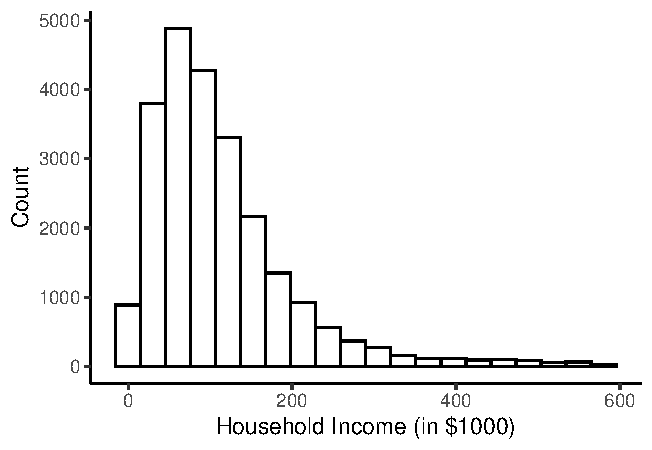
\includegraphics{./../../Output/hhi_hist.pdf}

Note that the distribution is skewed to the right due to a small number of outliers with really high incomes. 

\section{Measures of Central Tendency}

While a frequency distribution table or a histogram is a good way to learn about a variable, we only sometimes want to present a long table or a figure. We want a single number that can summarize this variable. A few options:
\begin{itemize}
\item[] \textit{{Mean}}:  the average value
\item[] \textit{{Median}}: the middle value 
\item[] \textit{{Mode}}: the most frequent value
\end{itemize} 

To calculate the median, you find the middle value. If the number of observations is even, you take the average of the two middle values. 

Mean and median are frequently employed in applied work. While the mean suffices for most purposes, it is more sensitive to outliers than the median because it considers all values, not just the middle values. For the distribution of household income above, the mean is \$112,900, and the median is \$91,600. Mean earnings are higher than the median, reflecting that the mean is pushed upwards as it is more affected by the outliers with really high incomes in the data. 

To calculate the mean, you add up all the observations and divide by the number of observations. A sample mean is usually denoted by $\bar{X}$ and can be calculated as:

$$ \bar{X} = \frac {\sum_{i=1}^n X_i}{n} $$ 

Here $n$ is the sample size. 

The population mean is denoted by $\mu$. \\

\fbox{\begin{minipage}{\textwidth}
Some things to note about the mean: 

\begin{itemize}
\item $\sum_{i=1}^n X_i = n \bar{X}$ 
\item Deviations from the mean are always zero
$$ \sum_{i=1}^n (X_i-\bar{X}) =  \sum_{i=1}^n X_i - n \bar{X} = n \bar{X}- n \bar{X}=0 $$
\item We can always write
$$ \bar{X} = \frac {\sum_{i=1}^n X_i}{n} = \frac{1}{n}\sum_{i=1}^n X_i = \sum_{i=1}^n \frac{X_i}{n} $$
\end{itemize}
\end{minipage}} \\ 

\subsection*{Mean from Grouped Data}

If data are grouped, we can use the frequency distribution table to calculate the mean.  In particular, for $K$ groups, we use the following formula: 

$$ \bar{X} = \frac{\sum_{k=1}^K n_k X_k}{n} = \sum_{k=1}^K f_k X_k $$

 Example. Say, we have the following observations on a variable $X$:  $$1,1,3,3,3,4,5$$ One way to find the mean:
 $$ \frac{1+1+3+3+3+4+5}{7} = \frac{20}{7}  $$
 
 Another way to find the mean:
 \begin{center}
\begin{tabular}{|c|c|p{1cm}|p{1cm}|}
\hline
$X_k$ & \hspace{0.5em} $n_k$ & \hspace{0.2em} $f_k$ & $f_k X_k$ \\
\hline
 1 & 2 & 2/7 & 2/7 \\
 \hline
3 &  3 & 3/7 & 9/7 \\
\hline
4 & 1 & 1/7 & 4/7 \\
\hline
5 &  1 & 1/7 & 5/7  \\
\hline
Total & 7 & 1 & 20/7 \\
\hline
\end{tabular}
 \end{center}
 
 Note that both approaches are equivalent, as all we do by using the frequency distribution table is group observations with the same values. 
 \begin{align*}
 	\frac{1+1+3+3+3+4+5}{7} &= \frac{(2\times 1)+(3\times 3)+(1\times 4)+(1 \times 5)}{7} \\
 	&= 2.\frac{1}{7} + 3.\frac{3}{7} + 4.\frac{1}{7}+ 5.\frac{1}{7}
 \end{align*}


\subsection*{Weighted Mean}
The \textit{weighted mean} of a set of data is given by:

$$ \bar{X} = \frac{\sum_{i=1}^n\omega_i X_i}{\sum_{i=1}^n \omega_i} $$

where $\omega_i$ is the weight of the $i^{th}$ observation. When weights sum up to 1 (i.e. \(\sum_{i=1}^n \omega_i=1\)) we can simply write the weighted mean as:

$$ \bar{X} = \sum_{i=1}^n\omega_i X_i$$ 

When we calculate the unweighted mean, we put equal weight on all observations in the data. However, sometimes we want to put a higher weight on some observations than others; in such cases, we use the weighted mean. 


\section{Percentiles}
The \textit{$P^{th}$ percentile} is a value such that $P$\% of observations are at or below that number. \\~\\
The 50th percentile is called the median. The 25th and 75th percentiles are called the 1st and 3rd quartiles, respectively.

\section{Measures of Variance}

Measures of central tendency tell us about the average observation in the data. However, it doesn't say anything about this variable's dispersion or variation. One way to learn about dispersion would be to look at the minimum and maximum values a variable takes. This is called the \textit{range} of the variable. Another way is to look at how far observations are away from the mean, so calculate the variance as follows. \\

\textit{Population Variance}
$$ \sigma_X^2 = \frac{1}{N} \sum_{i=1}^N (X_i-\mu_X)^2 $$
\textit{Sample Variance}
$$ S_X^2 = \frac{1}{n-1} \sum_{i=1}^n (X_i-\bar{X})^2 $$

If there is more dispersion in the data, the variance will be higher. This is because we calculate the mean by taking the average of square deviations from the mean. If many observations are further below or above the mean, the sum of square deviations will be larger. 

For the sample variance, the denominator is $n-1$ instead of $n$. This is because observations in the sample are closer to the sample mean than the population mean. The variance estimator uses the sample mean and hence underestimates the actual variance of the population. Dividing by $n-1$ instead of $n$ corrects for that bias. 

However, it isn't easy to interpret the variance since it is in \textit{squared units}. So we often convert the variance back to its original units by taking the square root of it. This quantity is called the standard deviation. 


\textit{Standard Deviation}
$$ \sigma_X = \sqrt{\sigma_X^2} \quad \quad S_X = \sqrt{S_X^2} $$ \\

\textit{Example.}
\begin{center}
	\begin{tabular}{|c|c|c|}
  \hline
  $X_i$ & $X_i-\mu$ & $(X_i-\mu)^2$ \\
  \hline
  2 & -3 & 9 \\
  \hline
  5 & 0 & 0 \\
  \hline
  8 & 3 & 9 \\
  \hline
  Total & 0 & 18 \\
  \hline
  \end{tabular}
\end{center}

We can calculate the variance as follows: 
$$ \sigma_X^2 = \frac{1}{3} \sum_{i=1}^3 (X_i-\mu_X)^2 = \frac{18}{3} = 6$$
The standard deviation is $\sigma_X = 2.45$. 

Note that we can use the frequency distribution table for grouped data to calculate the variance. In which case, 
$$ \sigma_X^2 = \sum_{k=1}^K f_k (X_k-\mu_X)^2 $$

 For the sample variance, we will need to do the $n-1$ correction as follows:
 $$ S_X^2 = \frac{n}{n-1} \sum_{k=1}^K f_k (X_k-\bar{X})^2 $$


\section{Z-Score}

Z-score is defined as:
$$ Z = \frac{X - \mu}{\sigma} $$
Z-score tells us how many standard deviations any particular observation is away from the mean.

Example. Say we have two hypothetical countries Mushroom Kingdom (MK) and Bowser's Kingdom (BK). Now say $$ \mu_{MK} = 50,000 \quad \quad  \mu_{BK} = 50,000 $$
$$ \sigma_{MK} = 3,000 \quad \quad  \sigma_{BK} = 5,000 $$

Someone earning \$ 45,000 in MK is $5000/ 3000 =1.66$ standard deviations below the mean. While someone earning \$ 45,000 in BK is $5000/ 5000 =1$ below the mean. Why the difference? Z-score standardizes both distributions and tells us how many people are between the person who earns 50K and 45K. 

\section{Correlation and Covariance}

While so far, we have been talking about describing one variable. Most often, we are interested in the relationship between two different variables. For instance, we might be interested in whether cars with better fuel economy have lower horsepower. To learn about such relationships, we can calculate the \textit{covariance}:

$$ \sigma_{XY} = \frac{1}{N}\sum_{i=1}^N (X_i-\mu_X)(Y_i-\mu_Y) \quad (Population) $$
$$ S_{XY} = \frac{1}{n-1}\sum_{i=1}^n (X_i-\bar{X})(Y_i-\bar{Y}) \quad (Sample) $$

Covariance indicates whether there is a positive or negative relationship between two variables. 

Why does this formula work? If it is, in fact, true that there is a negative relationship between fuel economy as measured by MPG and horsepower. Then for many observations in our data, $(X_i-\mu_X)(Y_i-\mu_Y)$ will be negative. $(X_i-\mu_X)(Y_i-\mu_Y)$ is negative every time $X_i$ is above its mean but $Y_i$ is below its mean or vice versa. 

Similarly, $(X_i-\mu_X)(Y_i-\mu_Y)$ is positive for any observation if both $X_i$ and $Y_i$ are above the mean. The covariance is positive if $(X_i-\mu_X)(Y_i-\mu_Y)$ is positive on average. If there is no clear relationship between the two variables, for some observations, $(X_i-\mu_X)(Y_i-\mu_Y)$ will be negative, while for some, it will be positive, leading the covariance to go towards 0. 

In other words, if two variables tend to be above average at the same time or below average at the same time, then we add a positive number to the numerator for the covariance for most observations, increasing the covariance. If they have nothing to do with each other, we add a positive number sometimes and a negative number other times, canceling each other and giving us a covariance of 0. 

The upper and lower limits for the covariance depend on the variances of the variables involved. These variances, in turn, can vary with the scaling of the variables, so even a change in the units of measurement can change the covariance. Thus, covariance is only helpful in finding the direction of the relationship between two variables and not the magnitude. 

We can obtain the \textit{correlation coefficient} of two variables by dividing the covariance of these variables by the product of the standard deviations of both variables. Correlation also indicates the strength of the relationship in addition to the direction.
$$ \rho_{XY} = \frac{ \sigma_{XY}}{\sigma_X \sigma_Y}  \quad (Population) $$
$$ r_{XY} = \frac{ S_{XY}}{S_X S_Y} \quad (Sample) $$

\fbox{\begin{minipage}{\textwidth}
Things to note about the correlation coefficient:
\begin{itemize}
\item Measures the strength and direction of the linear relationship between two variables
\item Bounded between $-1$ and $1$
\item If $\rho=0$, there is no linear relationship between the two variables. If $\rho=1$ or $\rho=-1$, there is a perfect linear relationship.
\item If $\rho>0$, then when $X$ is above (below) $\bar{X}$, $Y$ is above (below) $\bar{Y}$.
\item If $\rho<0$, then when $X$ is above (below) $\bar{X}$, $Y$ is below (above) $\bar{Y}$. 
\end{itemize}
\end{minipage}}
\vspace{1em}

Finally, correlation is not causation! Particularly for two reasons:
\begin{itemize}
\item[1.] Reverse causality: A high correlation between education and household income could come from either ``more education $\rightarrow$ higher household income'' or ``higher household income $\rightarrow$ more education.''
\item[2.] Other factors: It could be another factor like generational wealth is correlated with \underline{both} the likelihood of getting more education and having a higher household income. 
	
\end{itemize}


\end{document}